\section{Example of a game}

%\begin{figure}[h]
%\begin{center}
%    \includegraphics[width=11cm]{nom-du-fichier-image}
%\end{center}
%    \caption{phrase de legende pour limage}
%    \label{nom de la reference latex vers limage si on veut la citer dans le texte}
%\end{figure}

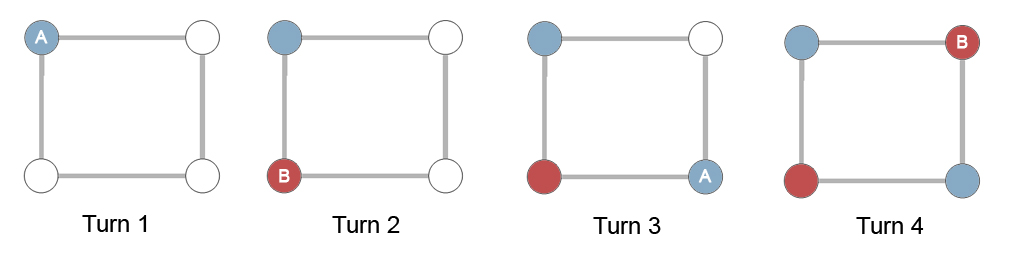
\includegraphics[width=10cm]{graphPER.jpg}

In the first part shown in the first picture, we see that the graph is 2-colorable. But during this game, Bob did not choose to play the worst choices.

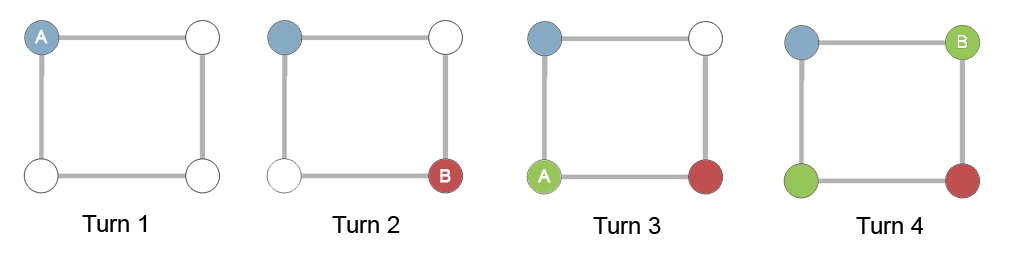
\includegraphics[width=10cm]{graphPER2.jpg}

During the second game, Bob decided to play a bad choice for Alice. We see immediately that despite the 2-colorable graph, we used three colors here. You see that the classical coloringof of a graph and the coloring game have very different consequences.